\begin{singlespacing}
\chapter{Context: theory and experiment}
\label{chapter:context}
%
\begin{epigraphs}
\qitem{%
The idea that theorems follow from the postulates does not correspond to simple
observation.
If the Pythagorean theorem were found to not follow from the postulates, we
would again search for a way to alter the postulates until it was true.
Euclid's postulates came from the Pythagorean theorem, not the other way.}%
{Richard~Hamming,
\textit{The Unreasonable Effectiveness of Mathematics},
1980~\cite{hamming1980unreasonable}}
\qitem{%
One geometry can not be more true than another; it can only be more convenient.
Geometry is not true, it is advantageous.}%
{Robert~M.~Pirsig,
\textit{Zen and the Art of Motorcycle Maintenance},
1974~\cite{pirsig1999zen}}
\end{epigraphs}
\end{singlespacing}

\begin{singlespacing}
\section{The Standard Model and beyond}
%
\begin{epigraphs}
\qitem{%
One geometry can not be more true than another; it can only be more convenient.
Geometry is not true, it is advantageous.}%
{Robert~M.~Pirsig,
\textit{Zen and the Art of Motorcycle Maintenance},
1974~\cite{pirsig1999zen}}
\end{epigraphs}
\end{singlespacing}

\TODO{Standard Model past present future}

\subsection{Particles}

\subsection{The Standard Model}

\subsection{Supersymmetric models}

\subsubsection{Minimal supersymmetric models}
Lightest Supersymmetric Particle (LSP)


\subsubsection{Guage Mediated Supersymmetry Breaking}
Gauge Mediated Supersymmetry Breaking (GMSB)



\begin{singlespacing}
\section{The \atlas\ Experiment}
%
\begin{epigraphs}
\qitem{%
if observing outer space gives us a view of the past, observing inner space
would surely give us a glimpse into the future - would be interesting if NASA
made a telescope for that%
}%
{Ken~M,
\textit{Comment: Yahoo! News},
2012~\cite{kenm2012inner}}
\end{epigraphs}
\end{singlespacing}

Towards explaining the main result of this thesis,
a search for effects from supersymmetric models in
\atlas~\cite{atlas2022searches},
we first some relevant facts about the \atlas\ detector ---
its design and history.

The \atlas\ detector was not delivered in a preordained form.
It was designed with intent to provide maximally useful and novel data within
real-world cost budgets.
Within general purpose utilities, \atlas' designs aimed to construct a
detector that could
\begin{itemize}
\item find the Higgs boson (which was predicted but yet unseen),
\item precisely measure known massive objects ($W$, $Z$, and $t$),
\item discover new (supersymmetric) particles~\cite{atlas1999design1}.
\end{itemize}
We now review these three goals with the subsequent news from \atlas'
operations.

\paragraph{Find the Higgs boson.}
Prior to \atlas' construction, the Higgs boson mass (and existence) was
poorly known, but loosely constrained by results like
$m(H) \gtrsim 90\,\eV[G]$ from searches at the
Large Electron–Positron Collider (LEP),
$m(H) = 76^{+85}_{-47}\,\eV[G]$ from other data on the electroweak sector,
and $m(H) \lesssim 1\,\eV[T]$ from theoretical unitarity arguments~\cite{
atlas1999design2,
ghinculov1998perturb,
lep1999ewk
}.

The Higgs boson couples to an extraordinary variety of fundamental particles.
For its discovery alone, \atlas' designers achieved sensitivity across the
entire $100$ to $1000\,\eV[G]$ window by targetting decays including
$H\to b\bar b$,
$H\to \gamma\gamma$,
$H\to ZZ^* \to 4\ell$, and
$H\to ZZ \to \ell\ell\nu\nu$;
these channels demand precise measurements of leptons, photons, and
$b$-jets, as well as sensitivity to the missing transverse momentum of
invisible neutrinos for $ZZ \to \ell\ell\nu\nu$ decays at the very highest
masses.

Both \atlas\ and \cms\ have now found a Higgs boson candidate at
$m(H) = 125\,\eV[G]$~\cite{
atlas2012higgs,
atlas2012combined,
cms2012higgs
}
and confirmed all of its tested Standard Model properties~\cite{
combined2016higgs,
atlas2022ten,
cms2022ten
}
such as its production mechanisms, decay rates,
spin, and parity~\cite{
HIGG-2013-01,
HIGG-2013-17,
HIGG-2014-06
}.

\paragraph{Precisely measure known massive objects.}
Other than the Higgs boson, the heavy Standard Model resonances are the
$W$ and $Z$ bosons and the top quark.
All of these are produced at high rates in LHC proton-proton collisions,
and present opportunities for \atlas\ to measure their properties
(such as masses and production cross-sections) with unprecedented precision.

Sensitivity to hadronic momenta is crucial,
both directly to measure heavy hadronic decays
(like $t \rightarrow bq\bar{q}$),
and indirectly for the missing transverse momenta from semi-invisible
leptonic decays (like $W \to \ell\nu$).
Since individual hadron identities are less relevant to these measurements,%
\footnote{%
Rare decays like
$W^\pm\rightarrow \pi^\pm \gamma$ or $W^\pm\rightarrow \pi^\pm \pi^+ \pi^-$
could give clean signals, but are not competitive due to their
tiny production rates and difficult identification~\cite{
cdf1996search,
mangano2014wpiy,
cms2021wpiy
}.%
}
it makes sense for \atlas' design to forfeit hadron identification systems
in favour of precise calorimetry with total angular coverage.

\atlas\ has now produced a plethora of competitively precise measurements
of the heavy Standard Model~\cite{atlas2021summarysm},
including $m(W)$~\cite{atlas2018wmass} and
$m(t)$~\cite{atlas2022symmarytop, atlas2019topmass, TOPQ-2015-03},
but also details of differential cross-sections~\cite{
STDM-2016-11,
STDM-2016-14,
TOPQ-2018-15,
TOPQ-2016-10
}.
Rare processes have also been studied in new levels of detail,
including
electroweak diboson ($WW/WZ/ZZ$ etc.)~\cite{
STDM-2015-21,
STDM-2015-23,
STDM-2017-09
}
and triboson~\cite{
STDM-2016-06,
STDM-2017-22,
STDM-2019-09
},
and rare top processes
($\ttbar Z$, $\ttbar W$ etc.)~\cite{
TOPQ-2013-05,
TOPQ-2018-01,
TOPQ-2020-03
},
These continue to not validate the Standard Model, and are aided by the lack of
new phenomena, which could have overpowered such rare signals.

\paragraph{Discover new (supersymmetric) particles.}
\TODO{
has discovery potential up to multi-TeV mass scales,
expect decays to knwon particles, so complements Higgs,
discovery and Standard Model measurements,
indeed search of this analysis benefits both from ZZ llvv and Hbb,
$\twoljets$ piggyback on the $ZZ \to \ell\ell\nu\nu$ channel
}

This is not a failure. It is a success.
Our goal is not to discover something that is not there, but to learn more
about nature.
The nonappearance of supersymmetric particles at the LHC is itself a discovery.

\TODO{
Decay to SM particles,
emphasis on missing transverse momentum.
...
Many SUSY searches, many other exotics searches, no convincing evidence for
new effects.
}



\subsection{Design}
Atlas is a Titan.
On the \cern\ Large Hadron Collider (LHC), \atlas\ is the largest detector
experiment, and alongside its majors neighbours
\cms~\cite{cms2008experiment},
\lhcb~\cite{lhcb2008experiment},
and ALICE~\cite{alice2008experiment}
it is a multi-kilotonne beast,
and a wonder of scientific engineering~\cite{
atlas2008experiment,
atlas1999design1,
atlas1999design2
}.

% design goals

Our search paper~\cite{atlas2022searches} contains concise and standard
descriptions of the \atlas\ detector and its relevant components.
Through its many inexact reproductions in past \atlas\ publications, the text
of these descriptions has become so highly refined that my attempts to improve
upon it would be in vain.
Instead, this section quotes our published text with explanatory commentary.

\begin{displayquote}
``%
The ATLAS detector~\cite{PERF-2007-01} is a multipurpose particle detector with
a forward--backward symmetric cylindrical geometry and a near $4\pi$ coverage
in solid angle.%
\footnote{%
``ATLAS uses a right-handed coordinate system with its origin at the nominal
interaction point (IP) in the centre of the detector and the $z$-axis along the
beam pipe.
The $x$-axis points from the IP to the centre of the LHC ring, and the $y$-axis
points upwards.
Cylindrical coordinates $(r,\phi)$ are used in the transverse plane, $\phi$
being the azimuthal angle around the $z$-axis.
The pseudorapidity is defined in terms of the polar angle $\theta$ as
$\eta = -\ln \tan(\theta/2)$.
Angular distance is measured in units of
$\Delta R \equiv \sqrt{(\Delta\eta)^{2} + (\Delta\phi)^{2}}$.%
''~\cite{atlas2022searches}
}
It consists of an inner tracking detector surrounded by a thin superconducting
solenoid providing a $2\,\mathrm{T}$ axial magnetic field, electromagnetic and
hadronic calorimeters, and a muon spectrometer.%
''~\cite{atlas2022searches}
\end{displayquote}

Figure~\ref{fig:atlas_cutaway}.

Inner detector~\ref{sec:atlas_inner}

Calorimeter systems~\ref{sec:atlas_calo}

Muon chambers~\ref{sec:atlas_muon}

Trigger~\ref{sec:atlas_trigger}

Software and data~\ref{sec:atlas_software_data}


\begin{figure}[tp]
\centering
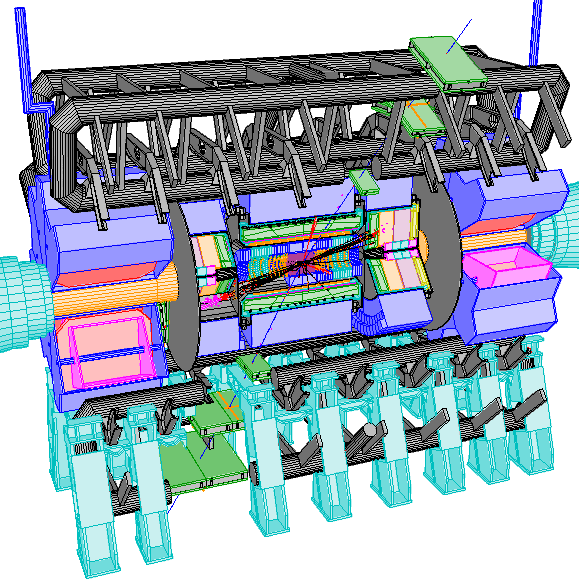
\includegraphics[width=0.6\textwidth]{figures/atlas_cutaway_volume_1.pdf}
\caption[
A central slice of \atlas' design
]{%
A central slice of \atlas' design, reproduced from~\cite{atlas1999design1},
including a simulated event that interacts with several sensitive subsystems.
}
\label{fig:atlas_cutaway}
\end{figure}


\subsection{Inner detector}
\label{sec:atlas_inner}
\TODO{inner detector}
\begin{displayquote}
``%
The inner tracking detector covers the pseudorapidity range $|\eta| < 2.5$.
It consists of silicon pixel, silicon microstrip, and transition radiation
tracking detectors.
An additional layer of silicon pixels, the insertable
B-layer~\cite{ATLAS-TDR-19, PIX-2018-001}, was installed before Run~2.%
''~\cite{atlas2022searches}
\end{displayquote}

\TODO{upgraded with IBL}

\subsection{Calorimeters}
\label{sec:atlas_calo}
\TODO{calo}
\begin{displayquote}
``%
Lead/liquid-argon (LAr) sampling calorimeters provide electromagnetic (EM)
energy measurements with high granularity.
A steel/scintillator-tile hadron calorimeter covers the central pseudorapidity
range ($|\eta| < 1.7$).
The endcap and forward regions are instrumented with LAr calorimeters for both
the EM and hadronic energy measurements up to $|\eta| = 4.9$.%
''~\cite{atlas2022searches}
\end{displayquote}

The `A' in \atlas\ does not stand for Argon, but perhaps it should.


\subsection{Muon system}
\label{sec:atlas_muon}
\TODO{muon system}
\begin{displayquote}
``%
The muon spectrometer surrounds the calorimeters and is based on three large
superconducting air-core toroidal magnets with eight coils each.
The field integral of the toroids ranges between $2.0$ and
$6.0\,\mathrm{T\kern-0.15ex m}$ across most of the detector.
The muon spectrometer includes a system of precision chambers for tracking and
fast detectors for triggering.%
''~\cite{atlas2022searches}
\end{displayquote}


\subsection{Trigger}
\label{sec:atlas_trigger}
\TODO{L1 HLT (L2, event thing)}
\TODO{trigger}
\begin{displayquote}
``%
A two-level trigger system is used to select events.
The first-level trigger is implemented in hardware and uses a subset of the
detector information to accept events at a rate below $100\,\mathrm{kHz}$.
This is followed by a software-based trigger that reduces the accepted event
rate to $1\,\mathrm{kHz}$ on average depending on the data-taking conditions.%
''~\cite{atlas2022searches}
\end{displayquote}


\subsection{Software and data}
\label{sec:atlas_software_data}
\TODO{how do we predict data?}
\TODO{software and data}
\begin{displayquote}
``%
An extensive software suite~\cite{ATL-SOFT-PUB-2021-001} is used in the
reconstruction and analysis of real and simulated data, in detector operations,
and in the trigger and data acquisition systems of the experiment.%
''~\cite{atlas2022searches}
\end{displayquote}


\TODO{discuss collisions, pileup, met}

\TODO{LHC runs}
